% =====================================================================
% Results: (1) multi-seed synthetic validation that the harness recovers
% planted structure; (2) N-modality generality; (3) real cohort as an
% integration test. Figures: figures/{taxonomy,complementarity3}.pdf
% =====================================================================

\section{Results}
\label{sec:results}

\subsection{Validation: the harness recovers planted structure}
\label{sec:validation}
We validate on synthetic echo/ECG data with planted structure---echo encodes LVEF strongly, ECG
weakly, except an $\approx$18\% subset where echo is uninformative so ECG must carry the
signal---training one Ridge probe on the full embeddings and masking at inference; splits are
stratified by the gate and independent of data generation (test-set HFrEF prevalence held in a sane
band). Across \textbf{12 seeds} the harness robustly recovers the planted attribution: echo's
leave-one-out value is $5.5{\pm}0.7$ MAE vs.\ $1.8{\pm}0.5$ for ECG, echo is the more valuable
modality in \textbf{all 12} seeds, and it takes $0.67{\pm}0.04$ of per-example wins while ECG
correctly wins on the planted complementary subset. The failure taxonomy (Fig.~\ref{fig:taxonomy})
shifts from mostly \emph{correct} under full inference to many \emph{critical} (gate-flipping) errors
when echo is dropped. We also report the loud-vs-silent split per modality; here the two are
comparable ($0.31{\pm}0.07$ silent when echo is dropped vs.\ $0.32{\pm}0.10$ for ECG, with the
ordering flipping across seeds). That is the intended behaviour: value and detectability are
\emph{separate} axes the harness measures, not an asymmetry it assumes---the most valuable modality
need not be the most dangerous to lose.

\begin{figure}[t]
\centering
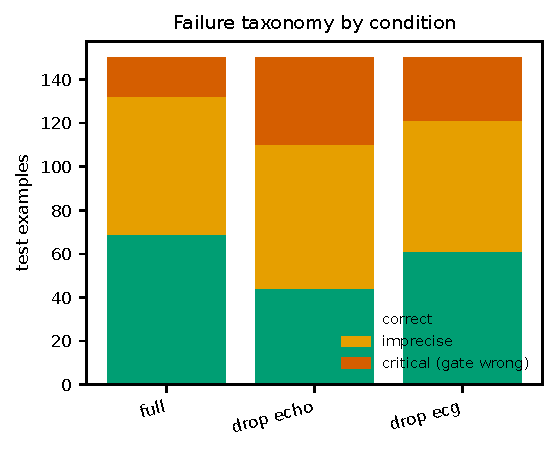
\includegraphics[width=0.58\linewidth]{figures/taxonomy.pdf}
\caption{Failure taxonomy by condition (representative seed; gate prevalence held healthy by
stratified splitting). Full-modality inference is mostly \emph{correct}; dropping echo introduces
many \emph{critical} gate-flipping failures---counts, not just MAE, make the clinically actionable
errors explicit.}
\label{fig:taxonomy}
\end{figure}

\subsection{Generality to $N$ modalities}
\label{sec:generality}
With only two modalities, per-example attribution is partly degenerate (dropping one equals using
the other), so we exercise the general path on a three-modality instance (echo, ECG, and a synthetic
``labs'' channel; \mbox{$n{=}225$} test). The harness returns a genuine $3{\times}3$ complementarity
matrix (Fig.~\ref{fig:matrix3}): echo solo reaches MAE $9.7$ vs.\ $12.9$ and $13.4$ for ECG and
labs, every echo-containing pair ($\approx$8.3) beats the ECG+labs pair ($11.3$), and marginal
values ($3.8/0.9/0.7$) with per-example wins ($125/56/44$) recover the planted ordering---flagging
echo as \emph{irreplaceable} and ECG/labs as weak and partly redundant. The same call scales to any
$N$.

\begin{figure}[t]
\centering
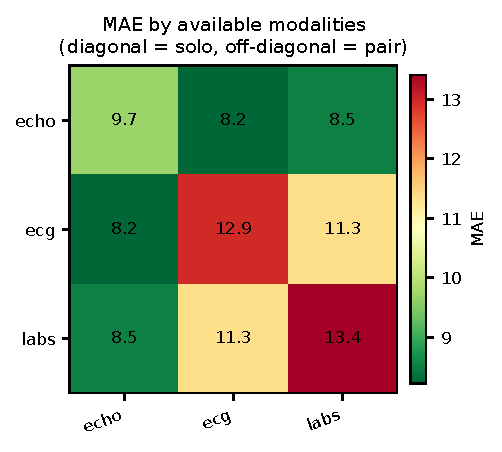
\includegraphics[width=0.46\linewidth]{figures/complementarity3.pdf}
\caption{Complementarity matrix on a three-modality instance: test MAE with each modality alone
(diagonal) and each pair (off-diagonal); lower is better. Every echo-containing combination far
outperforms ECG+labs, identifying echo as irreplaceable. Non-trivial attribution of this kind
requires \mbox{$N{\ge}3$}.}
\label{fig:matrix3}
\end{figure}

\subsection{Real cohort: an integration test}
\label{sec:realdemo}
Instantiated on real frozen EchoJEPA + ECG embeddings, a cross-attention probe on the held-out test
split (\mbox{$n{=}245$}) reproduces the expected aggregate dropout (Table~\ref{tab:degradation}):
dropping echo (the ECG-only deployment) nearly doubles MAE ($10.28\rightarrow18.57$) in this single
run. We treat this as an \emph{integration test} of the end-to-end pipeline rather than a validation
of the framework's per-example views: the taxonomy, complementarity, and loud-vs-silent outputs of
\S\ref{sec:validation} need a per-example prediction dump that the data-access barriers of
\S\ref{sec:lessons} held back. The released harness produces all three on these embeddings the
moment that dump is available.

\begin{table}[t]
\centering
\caption{Real-cohort missing-modality degradation (single held-out run, \mbox{$n=245$}); same fused
checkpoint, one branch masked per condition.}
\label{tab:degradation}
\small
\begin{tabular}{@{}lcc@{}}
\toprule
\textbf{Inference condition} & \textbf{LVEF MAE}\,$\downarrow$ & \textbf{EF\,$\leq$\,40\% AUROC}\,$\uparrow$ \\
\midrule
Full (echo $+$ ECG)        & \textbf{10.28} & \textbf{0.766} \\
Echo dropped (ECG-only)    & 18.57          & 0.693 \\
ECG dropped (echo-only)    & 15.13          & 0.750 \\
\bottomrule
\end{tabular}
\end{table}
